\documentclass[11pt]{article}
\input{/Users/markwang/.preamble}
\begin{document}


\section*{Inferences in Regression and Correlation Analysis}


\subsection*{2.1 Inference Concerning $\beta_1$}


\begin{defn*}
	\textbf{Inference concerning $\beta_1$} Test concerning $\beta_1$ is of the form 
	\[
		\begin{cases*}
			\mathcal{H}_0: \beta_1 = 0\\
			\mathcal{H}_{\alpha}: \beta_1 \neq 0  
		\end{cases*}
	\]
	$\beta_1 = 0$ implies that there is no linear association between $Y$ and $X$. On assumption of gaussian noise, there is also no relation of any type between $Y$ and $X$, since probability of $Y$ are identical for all levels of $X$ 
\end{defn*} 


\begin{defn*}
	\textbf{Linear estimators} Least square estimator $\hat{\beta}_1$ is a linear estimator
	\[
		\hat{\beta}_1 = \sum_i k_i y_i \quad \quad k_i = \frac{x_i -\overline{x}}{\sum_j (x_j - \overline{x})^2}
	\]
	with properties
	\[
		\sum k_i = 0 \quad \sum k_i x_i = 1 \quad \sum k_i^2 = \frac{1}{S_{XX}}
	\]
	\begin{proof}
		Note
		\[
			\sum (x_i - \overline{x})(y_i - \overline{y}) = \sum (x_i - \overline{x})y_i - \sum (x_i - \overline{x})\overline{y} = \sum (x_i - \overline{x})y_i \quad \text{by $\sum (x_i - \overline{x}) = 0$}
		\]
		the result follows. Proof of properties are simple, i.e.
		\[
			\sum k_i = \sum_i \left( \frac{x_i - \overline{x}}{\sum_j (x_j - \overline{x})^2} \right) 
			= \frac{1}{\sum_j (x_j - \overline{x})^2} \sum_i (x_i - \overline{x}) = 0
		\]
		For second property
		\[
			\sum k_i x_i 
			= \frac{1}{\sum_j (x_j - \overline{x})^2} \sum_i (x_i - \overline{x}) x_i 
			= \frac{1}{S_{XX}} \sum_i x_i^2 - n\overline{x}^2
			= \frac{1}{S_{XX}} S_{XX}
			= 1
		\] 
	\end{proof}
\end{defn*}

\begin{defn*}
	\textbf{Sampling distribution of $\hat{\beta}_1$} The sampling distribution of $\hat{\beta}_1$ refers to different values of the estimator obtained with repeated sampling when the levels of the predictor variable $X$ are held constant from sample to sample. Given $\hat{\beta}_1$ 
	\[
		\hat{\beta}_1 = \frac{\sum (x_i - \overline{x})(y_i - \overline{y})}{\sum (x_i - \overline{x})^2}
	\]
	The sampling distribution of $\hat{\beta}_1$ is \textbf{normal} with mean and variance,
	\[
		\E(\hat{\beta}_1 | X) = \beta_1 \quad Var(\hat{\beta}_1 | X) = \frac{\sigma^2}{\sum (x_i - \overline{x})^2} = \frac{\sigma^2}{S_{XX}}
	\]
	\[
		\hat{\beta}_1 \sim \norm(\beta_1, \frac{\sigma^2}{S_{XX}})
	\]
	\begin{proof}
		$ $\\
		\begin{enumerate}
			\item \textbf{Mean and variance}
			\[
				\E(\hat{\beta}_1) = \E\{ \sum k_i y_i \} \overset{ind}{=} \sum (k_i \E\{y_i \}) = \sum k_i(\beta_0 + \beta_1 x_i) = \beta_0 \sum k_i + \beta_1 \sum k_i x_i = \beta_1
			\]
			\[
				Var(\hat{\beta}_1) = Var\left( \sum k_i y_i \right) = \sum k_i^2 Var(y_i) = \sum k_i^2\sigma^2 = \sigma^2 \sum k_i^2 = \frac{\sigma^2}{S_{XX}}
			\]
			with last step of both derivation given by properties of $\hat{\beta}_1$ as a linear estimator. 
			\item \textbf{Normality} of sampling distribution given by the fact that $\hat{\beta}_1$ is a linear combination of $y_i$s. Since $y_i \overset{i.i.d}{\sim} \norm(\beta_0 + \beta1 x_i , \sigma^2)$, the estimator is normaly distributed because it is a linear combination of independent normal random variables
			\item \textbf{Estimated variance} We can estimate the variance of $\hat{\beta}_1$ by substituting $\sigma^2$ (unknown) with its unbiased estimator MSE $s^2$
			\[
				s^2 (\hat{\beta}_1) = \frac{MSE}{S_{XX}} \quad \text{ where } \quad MSE = \frac{\sum e_i^2}{n-2}
			\]
			Note $s^2$ carries a denominator of $S_{XX}$, this is from the variance of $\hat{\beta}_1$, we are simply substituting the unknown $\sigma^2$ with $MSE$
		\end{enumerate}
	\end{proof}
\end{defn*}


\begin{defn*}
	\textbf{standardization of $\hat{\beta}_1$} \\
	Standardization of sampling distribution of $\hat{\beta}_1$ gives 
	\[
		Z =  \frac{\hat{\beta}_1 - \beta_1}{\sigma(\hat{\beta}_1)} = \norm(0, 1) \quad \text{ wher } \quad \sigma(\hat{\beta}_1) = \frac{\sigma}{\sqrt{S_{XX}}}
	\]
	Usually, have to estimate standard error $\sigma(\hat{\beta}_1)$ with $s(\hat{\beta}_1)$. Standardization where the denominator is an estimated standard error is called \textbf{studentized statistic}, given by
	\[
		T = \frac{\hat{\beta}_1 - \beta_1}{s(\hat{\beta}_1)} \sim t_{n-2} \quad  \text{ where } \quad s^2(\hat{\beta}_1) = \frac{MSE}{S_{XX}}
	\]
	\begin{proof}
		Assume proposition 
		\[
			\frac{\sum (\hat{e}_i)^2 }{\sigma^2} \sim \chi^2_{n-2}
		\]
		Then we have 
		\[
			\frac{\hat{\beta}_1 - \beta_1}{s(\hat{\beta}_1)} 
			= \frac{\hat{\beta}_1 - \beta_1}{\sigma(\hat{\beta}_1)} \Biggm/ \frac{s(\hat{\beta}_1)}{\sigma(\hat{\beta}_1)} 
			= \frac{\hat{\beta}_1 - \beta_1}{\sigma(\hat{\beta}_1)} \Biggm/ \sqrt{\frac{\sum e_i^2 S_{XX}}{(n-2) S_{XX} \sigma^2 }}
			\sim \frac{Z}{\sqrt{\chi^2_{n-2} \Big/ (n-2)}} 
			= t_{n-2}
		\]
	\end{proof}
\end{defn*}


\begin{defn*}
	\textbf{Confidence Interval and test for $\beta_1$} \\
	We use the previously derived distribution as a pivot
	\[
		\Pr\left(t_{\alpha/2, n-2} \leq \frac{\hat{\beta}_1 - \beta_1}{s(\hat{\beta}_1)} \leq t_{1-\alpha/2, n-2}\right) = 1-\alpha
	\]
	\[
		\Pr\left(\hat{\beta}_1 - s(\hat{\beta}_1)t_{1-\alpha/2, n-2} \leq \beta_1 \leq \hat{\beta}_1 + s(\hat{\beta}_1)t_{1-\alpha/2, n-2} \right) = 1-\alpha
	\]
	Hence the confidence interval is given by 
	\[
		\hat{\beta}_1 \pm s(\hat{\beta}_1)t_{1-\alpha/2, n-2} \quad \text{ where }\quad s^2(\hat{\beta}_1) = \frac{MSE}{S_{XX}}
	\]
	For 2-sided tests
	\[
		\begin{cases*}
			\mathcal{H}_0: \beta_1 = b\\
			\mathcal{H}_{\alpha}: \beta_1 \neq b\\  
		\end{cases*}
	\]
	We compute test statistics 
	\[
		t^* = \frac{\hat{\beta}_1 - b}{s(\hat{\beta}_1)} \quad \text{ and reject $\mathcal{H}_0$ if }  |t^*| > t_{1-\alpha/2, n-2}
	\]
\end{defn*}


\subsection*{2.2 Inference Concerning of $\hat{\beta}_0$}

\begin{defn*}
	\textbf{Sampling Distribution of $\hat{\beta}_0$} \\
	Given point estimator 
	\[
		\hat{\beta}_0 = \overline{y} - \beta_1 \overline{x}
	\]
	$\hat{\beta}_0$ refers to different values of $\beta_0$ that would be obtained with repeated sampling when levels of predictor variable $x$ are held constant from sample to sample. The \textbf{sampling distribution of $\hat{\beta}_0$} is \textbf{normal} with mean and variance
	\[
		\E(\hat{\beta}_0) = \beta_0 \quad \quad Var(\hat{\beta}_0) = \sigma^2 \left[ \frac{1}{n} + \frac{\overline{x}^2}{\sum (x_i - \overline{x})^2} \right] = \sigma^2 \left[ \frac{1}{n} + \frac{\overline{x}^2}{S_{XX}} \right]
	\]
	\begin{proof}
		\[
			\E(\hat{\beta}_0) 
			= \E(\overline{y}) - \E(\hat{\beta}_1 \overline{x}) 
			= \frac{1}{n} \sum \E(y_i) - \beta_1 \overline{x}
			= \beta_0 + \beta_1 \frac{1}{n}\sum x_i - \beta_1 \overline{x} = \beta_0
		\]
		\begin{align*}
			Var(\hat{\beta}_0)
			&= Var(\overline{y} - \hat{\beta}_1 \overline{x})\\
			&= Var(\overline{y}) + \overline{x}^2 Var(\hat{\beta}_1) - 2\overline{x} Cov(\overline{y}, \hat{\beta}_1) \\
			&= Var(\frac{1}{n}\sum y_i) + \frac{\sigma^2}{S_{XX}} - 2\overline{x} Cov(\frac{1}{n} \sum y_i , \sum_i k_i y_i )\\
			&= \frac{\sigma^2}{n^2} + \frac{\sigma^2}{S_{XX}} - 2\overline{x} \frac{1}{n} \sum k_i Cov(y_i, y_i)\\
			&= \frac{\sigma^2}{n^2} + \frac{\sigma^2}{S_{XX}} - 2\overline{x} \frac{\sigma^2}{n} \sum k_i \\ 
			&= \sigma^2 \left(\frac{1}{n} + \frac{\overline{x}^2}{S_{XX}} \right)
		\end{align*}
		The normality follows because $\hat{\beta}_0$ is also a linear estimator of $y_i$s. We can estimate $Var(\hat{\beta}_0)$ by replacing $\sigma^2$ with MSE, as before
		\[
			s^2(\hat{\beta}_0) = MSE \left[ \frac{1}{n} + \frac{\overline{x}^2}{S_{XX}} \right]
		\] 
	\end{proof}
\end{defn*}

\begin{defn*}
	\textbf{Standardization of $\hat{\beta}_0$} \\
	
	\[
		Z = \frac{\hat{\beta}_0 - \beta_0}{\sigma(\hat{\beta}_0)} \sim t_{n-2} \quad \text{ where }\quad \sigma^2(\hat{\beta}_0) =  \sigma^2 \left[ \frac{1}{n} + \frac{\overline{x}^2}{S_{XX}} \right]
	\]
	\[
		T = \frac{\hat{\beta}_0 - \beta_0}{s(\hat{\beta}_0)} \sim t_{n-2} \quad \text{ where } \quad s^2(\hat{\beta}_0) = MSE \left[ \frac{1}{n} + \frac{\overline{x}^2}{S_{XX}} \right]
	\]
\end{defn*}

\begin{defn*}
	\textbf{Confidence Interval for $\hat{\beta}_0$}\\
	\[
		\hat{\beta}_0 \pm s(\hat{\beta}_0) t_{1-\alpha/2, n-2} \quad \text{ where } \quad s(\hat{\beta}_0) = \sqrt{\frac{\sum e_i^2}{n-2}} \sqrt{\frac{1}{n} + \frac{\overline{x}^2}{S_{XX}}}
	\]
\end{defn*}



\begin{defn*}
	\textbf{Consideration about inference}
	\begin{enumerate}
		\item \textbf{Spacing of $x$ levels} Looking at variance of $\hat{\beta}_0$ and $\hat{\beta}_1$, the larger the spread in $x$ levels, the larger $S_{XX}$ and smaller the variance. 
	\end{enumerate}
\end{defn*}



\subsection*{2.4 Interval Estimation of $\E(Y | X = x^*)$, the population regression line}


\begin{defn*}
	\textbf{Mean estimation} Often times want to estimate mean for one or more probability distribution of $Y$. (i.e. mean $Y$ for low and high $X$ levels). Let $x^*$ be level of $X$ for which we want to estimate the mean response $\hat{y}^*$. The mean response is given by 
	\[
		\E(Y | X = x^*) = E(y^*) = \beta_0 + \beta_1 x^*
	\]
	The idea is that the expectation is a random variable because of the estimated correlation coefficients. We would want to do inference on the mean response. We have a point estimator of the the mean response
	\[
		\hat{y}^* = \hat{\beta}_0 + \hat{\beta}_1 x^*
	\]
	which is simply the estimated response from estimated correlation coefficients and regression function. Note $X = x^*$ is a known constant 
\end{defn*}


\begin{defn*}
	\textbf{Sampling Distribution of mean response estimator $\hat{y}^*$} \\
	The sampling distribution of $\hat{y}^*$ is \textbf{normal} with mean and variance 
	\[
		\E(\hat{y}^*) = \E(\hat{y}|X=x^*) = \beta_0 + \beta_1 x^* \quad \text{($= \E(y^*)$ so unbiased)}
	\]
	\[
		Var(\hat{y}^*) = Var(\hat{y}|X=x^*) = \sigma^2 \left[ \frac{1}{n} + \frac{(x^* - \overline{x})^2}{\sum (x_i - \overline{x})^2} \right] = \sigma^2 \left[ \frac{1}{n} + \frac{(x^* - \overline{x})^2}{S_{XX}} \right]
	\]
	\[
		\hat{y}^* = (\hat{y}|X=x^*) \sim \norm(\beta_0 + \beta_1 x^*, \sigma^2 \left[ \frac{1}{n} + \frac{(x^* - \overline{x})^2}{S_{XX}} \right])
	\]
	Note when $x^*=0$, $Var(\hat{y}^*)$ reduces to variance of $\hat{\beta}_0$. 
	\begin{proof}
		3 parts
		\begin{enumerate}
			\item \textbf{Normality} of $\hat{y}^*$ follows from the fact that it is composed of $\hat{\beta}_0$ and $\hat{\beta}_1$, both of which are linear estimators of $y_i$
			\item \textbf{Mean}
			\[
				\E(\hat{y}^*)=  \E\left( \hat{\beta}_0 + \hat{\beta}_1 x^* \right) = \E(\hat{\beta}_0) + x^* \E(\hat{\beta}_1) = \beta_0 + \beta_1 x^* = \E(y^*)
			\]
			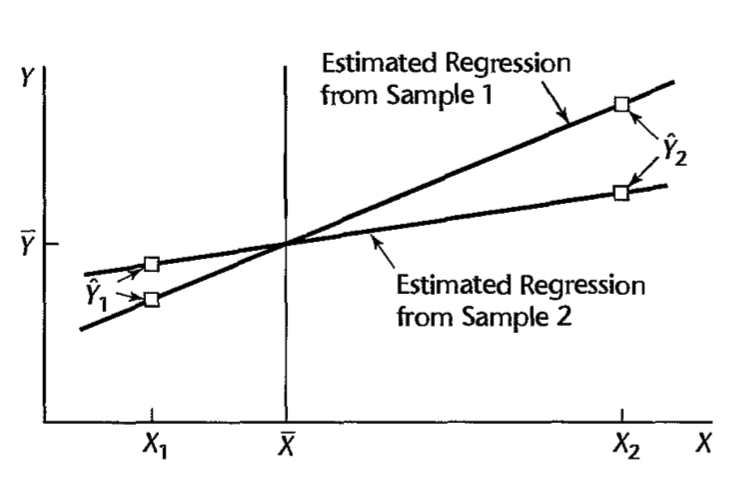
\includegraphics[width=\textwidth/2]{mean_response_var_plot}
			\item \textbf{Variance} 
			\begin{align*}
				Var(\hat{y} | X=x^*)
				&= Var(\hat{\beta}_0 + \hat{\beta}_1 x | X=x^*)\\
				&= Var(\hat{\beta}_0 | X=x^*) + (x^*)^2 Var(\hat{\beta}_1 | X = x^*) + 2x^* Cov(\hat{\beta}_0, \hat{\beta}_1 | X=x^*)
			\end{align*}
			with 
			\begin{align*}
				Cov(\hat{\beta}_0, \hat{\beta}_1 | X=x^*) 
				&= Cov(\overline{y} - \hat{\beta}_1 \overline{x} | X = x^*) \\
				&= Cov(\overline{y}, \hat{\beta}_1 | X = x^*) - \overline{x} Cov(\hat{\beta}_1, \hat{\beta}_1) \\
				&= 0 - \overline{x}Var(\hat{\beta}_1)\\
				&= \frac{-\overline{x}\sigma^2}{S_{XX}}
			\end{align*}
			So 
			\[
				Var(\hat{y} | X=x^*) = \sigma^2 \left( \frac{1}{2} + \frac{\overline{x}^2}{S_{XX}} \right) + (x^*)^2 \frac{\sigma^2}{S_{XX}} - \frac{2x^* \overline{x}\sigma^2}{S_{XX}} = \sigma^2 \left( \frac{1}{n} + \frac{(x^* - \overline{x})^2}{S_{XX}}\right)
			\]
			Idea is variability of $\hat{y}^*$ is affected by how far $x^*$ is from $\overline{x}$, via 
			\[
				(x^* - \overline{x})^2 = S_{XX}
			\]
			The further $x^*$ is from $\overline{x}$, the greater the variability. Note in plot, $x_1$ near $\overline{x}$, the fitted value $\hat{y}_1$ for two sample regression line (from 2 experiments) are close to each other; the fitted values $\hat{y}_2$ differ substantially due to the fact that $x_2$ is far from $\overline{x}$. In summary, 
			\begin{center}
				\textbf{variation in $\hat{y}^*$ value from sample to sample will be greater when $x^*$ is far from mean than when $x^*$ is near mean} 
			\end{center}
			We can substitute MSE for $\sigma^2$ to obtain $s^2(\hat{y}^*)$. The estimated variance is given by
			\[
				 s^2(\hat{y}^*) = MSE \left[ \frac{1}{n} + \frac{(x^* - \overline{x})^2}{S_{XX}} \right]
			\]
		\end{enumerate}
	\end{proof}
\end{defn*}

\begin{defn*}
	\textbf{Standardization of mean response estimator $\hat{y}^*$}\\
	\[
		Z = \frac{\hat{y}^* - (\beta_0 + \beta_1 x^*)}{\sigma(\hat{y}^*)} \sim \norm(0,1)
	\]
	note $\E(y^*) = \beta_0 + \beta_1 x^*$
	\[
		T = \frac{\hat{y}^* - (\beta_0 + \beta_1 x^*)}{s(\hat{y}^*)} \sim t_{n-2}
	\]
\end{defn*}

\begin{defn*}
	\textbf{Confidence Interval for $\hat{y}^*$}\\
	The $100(1-\alpha)\%$ confidence interval for $\E(Y|X=x^*)=\beta_0 + \beta_1 x^*$ is given by
	\[
		\hat{y}^* \pm s(\hat{y}^*) t_{1-\alpha/2, n-2} = (\hat{\beta}_0 + \hat{\beta}_1 x^*) \pm t_{1-\alpha/2, n-2} \sqrt{\frac{\sum e_i^2}{n-2}}\sqrt{ \frac{1}{n} + \frac{(x^* - \overline{x})^2}{S_{XX}} }
	\]
\end{defn*}


\begin{defn*}
	\textbf{Obervations}
	\begin{enumerate}
		\item variance of $\hat{y}^*$ is smallest when $x^* = \overline{x}$. So in an experiment to estimate mean response at a particular level $x^*$ of predictor variable, the \textbf{precision of the estimate is greatest} if (everything else remain equal) the observations on $X$ are spaced so that $\overline{x} = x^*$
		\item confidence interval for $\hat{y}^*$ not sensitive to moderate departures from assumption of error being normally distributed. The robustness in estimating mean response is related to robustness of Confidence interval for $\beta_0$ and $\beta_1$
	\end{enumerate}
\end{defn*}


\subsection*{2.5 Prediction of New Observations}

\begin{defn*} \textbf{Prediction of New Observations}
	\begin{enumerate}
		\item \textbf{Motivation}  Idea is that we have a model set up given a set of data, and we would want to extrapolate to new data points. The new observation $Y$ is viewed as the result of a new trial, independent of trials on which the regression analysis is based. Let level of $X$ be $x^*$ and the new observation $y^*_{new}$ (which is unknown, and which we want to characterize), assuming that the underlying regression model is still appliacble for basic sample data 
		\item \textbf{Estimate of mean response $\E(y^*)$ vs. Prediction of new response $y^*_{new}$ } \\
		In the former case, we estimate \textbf{mean of distribution of $Y$}. In latter case, we predict an \textbf{individual outcome} drown from the distribution of $Y$. Idea is we have to take into account of the fact that the majority of individual outcomes deviate from the mean response
	\end{enumerate}
\end{defn*}


\begin{defn*}
	\textbf{Prediction Interval for $y^*_{new}$ when parameter is known} \\
	Assume all parameters are known, we have $y^*$ follow a normal distribution 
	\[
		y^*_{new} \sim \norm(\beta_0 + \beta_1 x^*, \sigma^2)
	\]
	So we have confidence interval, 
	\[
		\left( \beta_0 + \beta_1 x^* \right) \pm \sigma z_{1-\alpha/2} 
	\]
\end{defn*}

\begin{defn*}
	\textbf{Prediction Interval for $y^*_{new}$ when parameter is unknown} \\
	When parameter is unknown, we must estimate regression parameters. We might want to estimate mean distribution of $Y$ with $\hat{y^*}$ and variance of distribution of $Y$ with MSE. 
	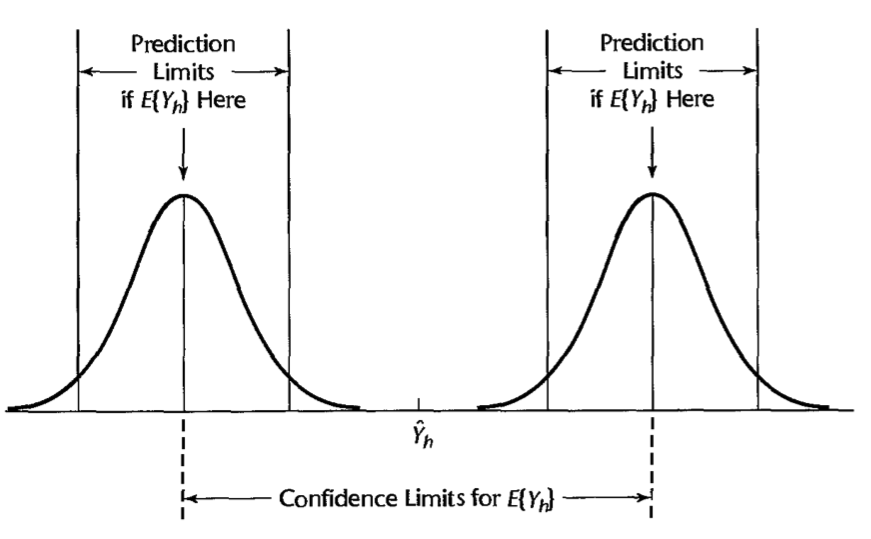
\includegraphics[width=\textwidth/2]{prediction_interval_conf_lim}  \\
	However, we cannot substitute these estimate into the previous distribution because $\E(y^*)$ is a random variable. Since we do not know the mean $\E(y^*)$, and only estiamte it by a confidence interval (shown previously), we cannot be certain of the distribution of $Y$. It could be anywhere along within its confidence intervals (for $\E\{Y_h\}$). Hence \textbf{prediction limit} for $y^*_{new}$ must take into account two elements
	\begin{enumerate}
		\item variation in possible location of distribution of $Y$ (i.e. sampling distributino of $\hat{y}^*$)
		\item variation within the probability distribution of $Y$ (namely $\sigma^2$, same as that of error terms')
	\end{enumerate}
	We can prove that
	\[
		\E(y^*_{new} - \hat{y}^*) 
		= \E(y_{new} - \hat{y}|X = x^*)
		= \E(\hat{\beta}_0 + \hat{\beta}_1 x^*) - \E(\hat{y}^*) 
		= 0
	\]
	\[
		Var(y^*_{new} - \hat{y}^*) 
		= Var(\hat{\beta}_0 + \hat{\beta}_1 x^*) + Var(\hat{y}^*)
		= \sigma^2 + \sigma^2 \left[ \frac{1}{n} + \frac{(x^* - \overline{x})^2}{S_{XX}} \right]
		= \sigma^2 \left[ 1+ \frac{1}{n} +\frac{(x^* - \overline{x})^2}{S_{XX}} \right]
	\]
	Note $Cov(y^*_{new}, \hat{y}^*) = 0$ by independence
	\[
		y^*_{new} - \hat{y}^* \, \sim \, \norm(0, \sigma^2 \left[ 1+ \frac{1}{n} +\frac{(x^* - \overline{x})^2}{S_{XX}} \right])
	\]
	An unbiased estimtor of the variance is given by 
	\[
		s^2(y^*_{new} - \hat{y}^*) = MSE \left[ 1+ \frac{1}{n} +\frac{(x^* - \overline{x})^2}{S_{XX}} \right]
	\]
	\textbf{Standardization of $y^*_{new}$} gives 
	\[
		T = \frac{y^*_{new} - \hat{y}^*}{s^2(y^*_{new} - \hat{y}^*)} \, \sim \, t_{n-2}
	\]
	The $(100-\alpha)\%$ \textbf{Prediction limit} for $y^*_{new}$ at $X=x^*$ is thus given by,
	\[
		(\hat{\beta}_0 + \hat{\beta}_1 x^*) \, \pm \, t_{1-\alpha/2, n-2} MSE \sqrt{1+ \frac{1}{n} +\frac{(x^* - \overline{x})^2}{S_{XX}} } 
	\]
\end{defn*}

\begin{defn*}
	\textbf{Comments}
	\begin{enumerate}
		\item prediction limit is subject to departure from normality of error term distributions
		\item A confidence interval represents an inference on a paramter and is an interval that is intended to cover the value of \textbf{parameter}. A prediction interval, is a statement about the value to be taken by a \textbf{random variable}, the new observation $y^*_{new}$
	\end{enumerate}
\end{defn*}
 

\subsection*{Confidence-band for Regression line} 

\begin{defn*}
	\textbf{Confidence-band} represents uncertainty in the estimate of regression line (i.e. $\E(Y) = \beta_0 + \beta_1 X$). Used to determine appropriateness of a fitted regression function. \
	\textbf{The Working-Hotelling} $1-\alpha$ confidence band for regression line has boundary values at any level $x^*$
	\[
		\hat{y}^* \pm Ws\{ \hat{y}^*\} \quad \text{ where } \quad W^2 = 2F_{1-\alpha, n-2}
 	\]
\end{defn*}


\subsection*{Analysis of Variance Approach to Regression Analysis}

\begin{defn*}
	\textbf{Partitioning Total sum of Squares} Idea is to partititon sums of squares and degree of freedom associated with response variable $Y$\\
	\begin{center}
		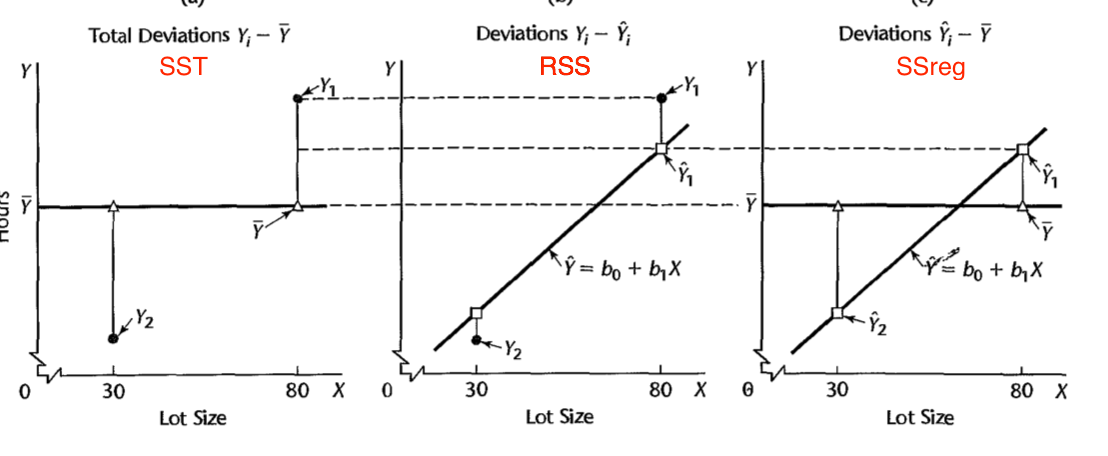
\includegraphics[width=\textwidth]{anova_simple_reg}
	\end{center}
	\begin{enumerate}
		\item \textbf{Total sum of squares} (SST) 
		\[
			SST = \sum (y_i - \overline{y})^2
		\]
		is a measure of uncertainty of $Y$, without taking $X$ into account
		\item \textbf{Residual sum of squares} (RSS, SSE)
		\[
			RSS = \sum (y_i - \hat{y}_i)^2
		\]
		is a measure of variation of $Y$, with $X$ taken into account. The greater variation of $Y$ around fitted regression line, the larger the $RSS$. 
		\item \textbf{Regression sum of squares} (SSR, SSreg)
		\[
			SSreg = \sum (\hat{y}_i - \overline{y})^2
		\]
		Alternatively we can expand and get to an equivalent expression 
		\[
			SSreg = \sum ((\hat{\beta}_0 - \hat{\beta}_1x_i) - (\hat{\beta}_0 + \hat{\beta}_1 \overline{x}))^2 
			= \hat{\beta}_1^2 \sum (x_i - \overline{x})^2
		\]
	\end{enumerate}
	SST can be broken down into 2 components, i.e. deviation of fitted value $\hat{Y}_i$ around mean $\overline{Y}$ and deviation of observed $Y_i$ around fitted regression line
	\begin{center}
		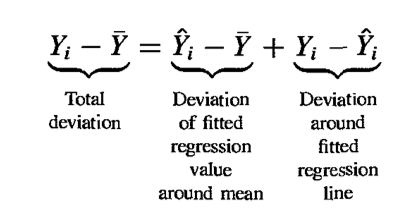
\includegraphics[width=\textwidth/2]{anova_partitioning}
	\end{center}
	The sum of these squared deviations have the same relationship!
	\[
		\sum (Y_i - \hat{Y})^2 = \sum (\hat{Y}_i - \overline{Y})^2 + \sum (Y_i - \hat{Y}_i)^2
	\]
	\[
		SST = RSS + SSreg
	\]
	\[
		\text{total variability} =\text{unexplained variability} + \text{variability explained by model}
	\]
	\begin{proof}
		\begin{align*}
			\sum (y_i - \overline{y})^2 
			&= \sum [(\hat{y}_i - \overline{y}) + (y_i - \hat{y}_i)]^2\\ 
			&= \sum (\hat{y}_i - \overline{y})^2 + \sum (y_i - \hat{y}_i)^2 + 2\sum(\hat{y}_i - \overline{y})(y_i - \hat{y}_i)\\
			&= SSreg + RSS 
		\end{align*}
		where 
		\begin{align*}
			2\sum(\hat{y}_i - \overline{y})(y_i - \hat{y}_i) 
			&= 2\sum \hat{y}_i (y_i - \hat{y}_i) - 2\overline{y}\sum (y_i - \hat{y}_i)\\
			&= 2\sum \hat{y}_i e_i - 2\overline{y} \sum e_i \\
			&= 0
		\end{align*}
	\end{proof}
\end{defn*}

\begin{defn*}
	\textbf{Break down of degress of freedom} 
	\begin{enumerate}
		\item SST has $n-1$ degrees of freedom (1 df is lost because sample mean $\overline{y}$ is used to estimate population mean)
		\item RSS has $n-2$  degrees of freedom (2 df lost because $\beta_0$ and $\beta_1$ are estimated)
		\item SSreg has $1$ degree of freedom. 
	\end{enumerate}
	\[
		n - 1 = 1 + (n - 2)
	\]
\end{defn*}

\begin{defn*}
	\textbf{Mean Squares} A sum of squares divided by its associated degree of freedom is mean square
	\[
		MSR = \frac{SSreg}{1} = SSreg \quad \quad MSE = \frac{RSS}{n-2}
	\]
	$MSE$ of an estimator measures the average of the squares of the errors or deviations, i.e. the difference between the estimator and what is estimated. $MSE$ is a measure of quality of estimator
\end{defn*}

\begin{defn*}
	\textbf{Analysis of Variance Table} displays breakdowns of total sum of squares and associated degrees of freedom
	\begin{center}
		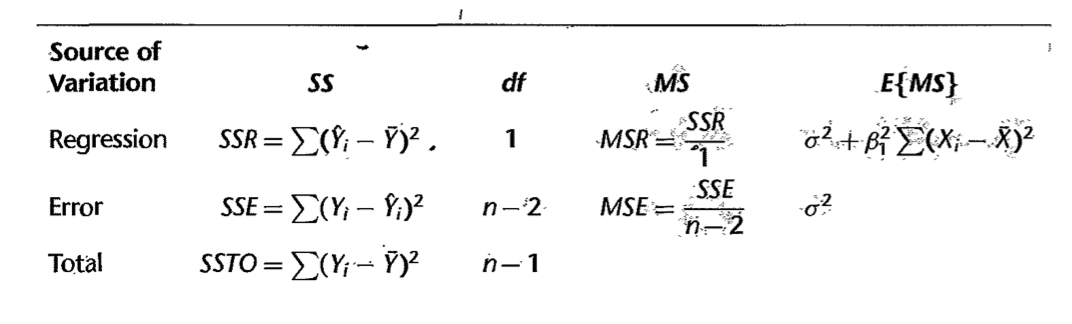
\includegraphics[width=\textwidth]{anova_table}
	\end{center}
\end{defn*}

\begin{defn*}
	\textbf{Expected Mean square} Expected value of a mean square is the mean of its sampling distribution and tells us what is being estimated by the mean square. 
	\begin{align*}
		\E(MSE) &= \sigma^2 \\
		\E(MSR) &= \sigma^2 + \beta_1^2 \sum (x_i - \overline{x})^2
	\end{align*}
	\begin{proof}
		Given 
		\[
			\frac{RSS}{\sigma^2} \sim \chi^2_{n-2}
		\]
		We have 
		\[
			\E(\frac{RSS}{\sigma^2}) = n-2 \quad \to \quad \E(\frac{RSS}{n-2}) = \E(MSE) = \sigma^2
		\]
		To prove $\E(MSR)$, we first note form of $SSreg$,
		\begin{align*}
			SSreg 
			&= \hat{\beta}_1^2 \sum (x_i - \overline{x})^2 \\
		\end{align*}
		to find its expected value, we first find 
		\[
			\E(\hat{\beta}_1^2) 
			= Var{\hat{\beta}_1} + (\E(\hat{\beta}_1))^2
			= \frac{\sigma^2}{S_{XX}} + \beta_1^2 
		\]
		Then we have 
		\[
			\E(SSreg) 
			= \E(\hat{\beta}_1^2) \sum (x_i - \overline{x})^2
			= (\frac{\sigma^2}{S_{XX}} + \beta_1^2 ) S_{XX}
			= \sigma^2 + \beta_1^2 S_{XX}
		\]
		Then we find mean squared regression 
		\[
			\E(MSR) = \E(\frac{SSreg}{1}) = \sigma^2 + \beta_1^2 S_{XX}
		\]
	\end{proof}
\end{defn*}


\begin{defn*}
	\textbf{$F$ test of $\beta_1 = 0$ versus $\beta_1 \neq 0$}\\
	To test for if there is a linear relationship between $X$ and $Y$,
	We can test for this with t test 
	\[
		T = \frac{\hat{\beta}_1 - 0}{\sigma / \sqrt{S_{XX}}} \sim t_{n-2} 
	\]
	Alternatively, to generalize the test to multiple regression, we can use $F$ test where test statistics is given by 
	\[
		F^* = \frac{MSR}{MSE} = \frac{SSreg}{RSS/(n-2)}
	\]
	Intuitively, larger values of $F^*$ (larger $MSR$) supports $H_{\alpha}$ and values of $F^*$ near 1 supports $H_0$. It can be shown that sampling distribution for $F^*$ is given by 
	\[
		F^* \sim F_{1, n-2}
	\]
	The test is then given by 
	\[
		\textbf{Reject if } F^* > F_{1-\alpha; 1, n-2} 
	\]
\end{defn*}

\begin{defn*}
	\textbf{Equivalence of $F$ test and $t$ test}\\
	Given $\alpha$ confidence level, $F$ test of $\beta_1 = 0$ versus $\beta_1 \neq 0$ is equivalent to two-sided t test 
	\begin{proof}
		\[
			F^* 
			= \frac{SSreg/1}{RSS/(n-2)}
			= \frac{\hat{\beta}_1 \sum (x_i - \overline{x})^2}{MSE}
			= \frac{\hat{\beta}_1 S_{XX}}{MSE}
		\]
		Note 
		\[
			s^2(\hat{\beta}_1) = \frac{MSE}{S_{XX}}
		\]
		we have 
		\[
			F^* = \left( \frac{\hat{\beta}_1^2 - 0}{s(\hat{\beta}_1)} \right)^2
			= (t^*)^2
		\]
		where $t$ is the t statistics
	\end{proof}
\end{defn*}


\subsection*{2.9 Descriptive Measures of \textbf{Linear Association} between $X$ and $Y$}

\begin{defn*}
	\textbf{Coefficient of Determination} \\
	\begin{enumerate}
		\item $SST$ measures variation in $Y$ without taken into account of $X$
		\item $RSS$ is a measure of variation in $Y$ when taken into account of $X$
		\item A natural measure of effect of $X$ in reducing variation in $Y$ is in the difference between $SST$ and $RSS$ as a proportion of total variation 
	\end{enumerate}
	The \textbf{coefficient of determination} $R^2$ is given by
	\[
		R^2= \frac{SST - RSS}{SST}= \frac{SSreg}{SST}
	\]
	with 
	\[
		0 \leq R^2 \leq 1
	\]
	$R^2$ can be interpreted as the proportionate reduction of total variation associated with use of $X$ predictor variable
\end{defn*}



\begin{defn*}
	\textbf{Coefficient of Correlation}\\ 
	A measure of linear association between $Y$ and $X$ when both $Y$ and $X$ are random is coefficient of correlation. 
	\[
		r = \pm \sqrt{R^2}
	\]
\end{defn*}


\subsection*{Dummy variable regression}




\end{document}